\documentclass{article}
\newcommand{\ImageWidth}{11cm}
\usepackage{tikz}
\usetikzlibrary{decorations.pathreplacing,positioning, arrows.meta}

\begin{document}         
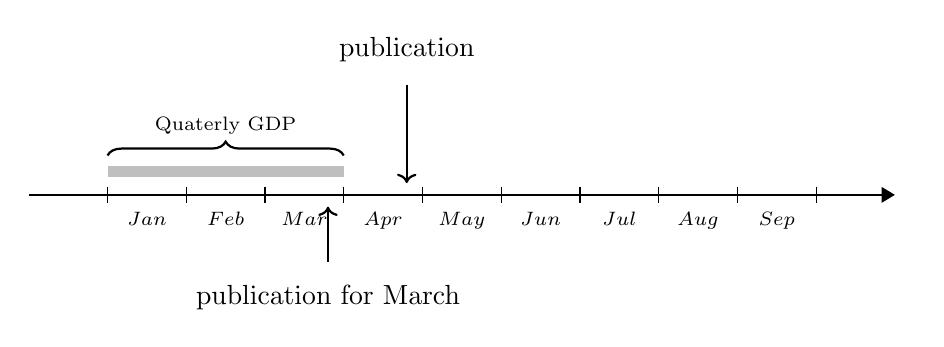
\begin{tikzpicture}
% draw horizontal line   
\draw[thick, -Triangle] (0,0) -- (\ImageWidth,0) node[font=\scriptsize,below left=3pt and -8pt]{ };

% draw vertical lines
\foreach \x in {1,...,10}
\draw (\x cm,3pt) -- (\x cm,-3pt);

\foreach \x/\descr in {1.5/Jan, 2.5/Feb, 3.5/Mar, 4.5/Apr, 5.5/May, 6.5/Jun, 7.5/Jul, 8.5/Aug,9.5/Sep}
\node[font=\scriptsize, text height=1.75ex,
text depth=.5ex] at (\x,-.3) {$\descr$};

% colored bar up
\foreach \x/\perccol in
{1/100,2/75,3/25}
\draw[lightgray, line width=4pt] 
(\x,.3) -- +(1,0);

% braces
\draw [thick ,decorate,decoration={brace,amplitude=5pt}] (1,0.5)  -- +(3,0) 
       node [black,midway,above=4pt, font=\scriptsize] {Quaterly GDP};
%\draw [thick,decorate,decoration={brace,amplitude=5pt}] (6,-.9) -- +(-1,0)
%       node [black,midway,font=\scriptsize, below=4pt] {Publication};

% time of publication
\node[align=center] at (4.8,1.85) {publication};
\draw [thick,->] (4.8,1.4) -- (4.8,0.15);
\node[align=center] at (3.8,-1.3) {publication for March};
\draw [thick,->] (3.8,-0.85) -- (3.8,-0.15);
\end{tikzpicture}


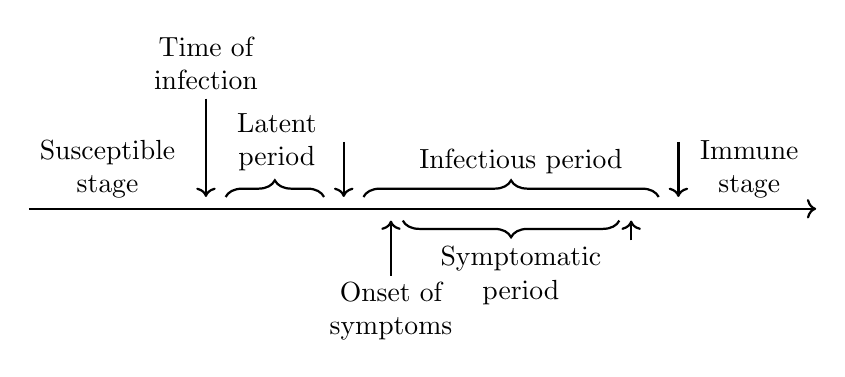
\begin{tikzpicture}[scale=1]
\node[align=center] at (1,0.5) {Susceptible\\stage};
\node[align=center] at (2.25,1.85) {Time of\\infection};
\draw [thick,->] (2.25,1.4) -- (2.25,0.15);
\node[align=center] at (3.15,0.85) {Latent\\period};
\draw [thick,decorate,decoration={brace,amplitude=6pt,raise=0pt}] (2.5,0.15) -- (3.75,0.15);
\draw [thick,->] (4,0.85) -- (4,0.15);
\node[align=center] at (6.25,0.6) {Infectious period};
\draw [thick,->] (8.25,0.85) -- (8.25,0.15);
\node[align=center] at (9.15,0.5) {Immune\\stage};
\draw [thick,decorate,decoration={brace,amplitude=6pt,raise=0pt}] (4.25,0.15) -- (8,0.15);
\draw [thick,->] (0,0) -- (10,0);
\draw [thick,->] (4.6,-0.85) -- (4.6,-0.15);
\draw [thick,->] (7.65,-0.4) -- (7.65,-0.15);
\draw [thick,decorate,decoration={brace,amplitude=6pt,raise=0pt,mirror}] (4.75,-0.15) -- (7.5,-0.15);
\node[align=center] at (6.25,-0.85) {Symptomatic\\period};
\node[align=center] at (4.6,-1.3) {Onset of\\symptoms};
\end{tikzpicture}

\end{document}